\documentclass{beamer}
\usetheme[hideothersubsections]{HRTheme}
\usepackage{beamerthemeHRTheme}
\usepackage{graphicx}
\usepackage[space]{grffile}
\usepackage{listings}
\usepackage{animate}
\lstset{language=SQL,
basicstyle=\ttfamily\footnotesize,
mathescape=true,
keywordstyle=\color{blue},
breaklines=true,
showspaces=false,
showstringspaces=false}
\usepackage[utf8]{inputenc}
\usepackage{color}
\newcommand{\red}[1]{
\textcolor{red}{#1}
}
\newcommand{\ts}{\textbackslash}

\title{ACID, Transaction Management and Conccurrency Control }

\author{ }

\institute{Hogeschool Rotterdam \\ 
Rotterdam, Netherlands}

\date{}

\begin{document}
\maketitle

\SlideSection{Introduction}
\SlideSubSection{Lecture topics}
\begin{slide}{
\item ACID.
\item Transaction Management.
\item Concurrency Control.
}\end{slide}

\SlideSection{Transactions and Concurrency}
\SlideSubSection{Reasons}
\begin{slide}{
\item \emph{Concurrent} execution essential for good DBMS performance.
\item Disk accesses frequent, relatively slow. Important to keep the cpu busy by working on several user programs concurrently.
\item Client application may carry out many operations on the data retrieved from the database.
\item DBMS is only concerned about what data is read/written from/to the database.
\item A \textit{transaction} is the DBMS’s abstract view of a user program:  a sequence of \red{reads} and \red{writes}.
}\end{slide}


\SlideSubSection{Transactions and Concurrency}
\begin{slide}{
\item Users submit transactions, and can think of each transaction as executing by itself.
\begin{itemize}
	\item \emph{Concurrency} is achieved by the DBMS: reads/writes of DB objects of various transactions.
	\item transaction must leave the database in a consistent state if the DB is consistent when the transaction begins.
	\item DBMS does not need to understand the semantics of the data.  (e.g. how the interest on a bank account is computed).	
\end{itemize}
\item Issues:  Effect of interleaving transactions, and crashes.
}\end{slide}

\SlideSubSection{The ACID properties }
\begin{slide}{
\item A RDBS ensures this four properties of a transaction:
\begin{itemize}
	\item \textbf{Atomicity}: states that database modifications must follow an all or nothing rule.
	\pause
	\item \textbf{Consistency}: states that only valid data will be written to the database.
	\pause
	\item \textbf{Isolation}: requires that multiple transactions occurring at the same time not impact each others execution.
	\pause
	\item \textbf{Durability}: ensures that any transaction committed to the database will not be lost. 	
\end{itemize}
}\end{slide}

\SlideSubSection{Atomicity of Transactions}
\begin{slide}{
\item A transaction either \red{commit} after completing all its actions or \red{abort} after executing some actions.
\item A user can think of a transaction as always executing all its actions in one step, or not executing any actions at all.
\item DBMS logs all actions so that it can undo the actions of aborted transactions.		
}\end{slide}

\SlideSection{Example of a Transaction}
\begin{frame}[fragile]{Transaction}
\begin{lstlisting}
BEGIN;
UPDATE ships SET name = 'Alpha'
	WHERE name = 'Oleg';
SAVEPOINT my_savepoint;
UPDATE ships SET integrity = 30
	WHERE name = 'Alpha';
-- oops ... forget that and update Beta 
ROLLBACK TO my_savepoint;
UPDATE ships SET integrity = integrity + 10
	WHERE name = 'Beta';
COMMIT;		
\end{lstlisting}
\red{When are those updates valid states for other actions?}  
\end{frame}	


\SlideSubSection{Transactions}
\begin{slide}{
\item We simplify transaction queries for readability in our next example  
\pause
\item Consider those two transactions:
\begin{itemize}
	\item T1:	BEGIN   ship1.energy = ship1.energy - 10, ship2.shields = ship2.shields + 10    COMMIT
	\item T2:	BEGIN   ship1.energy = 1.05 * ship1.energy,  ship2.shields = 1.05 * ship2.shields   COMMIT
	
\end{itemize}
\item The first transaction is using \texttt{ship1} energy to recharge \texttt{ship2} shields.  
\item Both the energy and the shields are being recharged by a nearby generator which recharge by 5\% of the total amount.
\item \red{How are those transaction scheduled?}	
}\end{slide}


\SlideSubSection{Transactions}
\begin{slide}{
\item Possibility 1:
\begin{table}
	\tiny
	\begin{tabular}{l|l}
		T1 & T2\\
		\hline
		s1.energy = s1.energy - 10 & \\
		& s1.energy = 1.05 * s1.energy \\
		s2.shield = s2.shields + 10 & \\
		Commit & \\
		& s2.shields = 1.05 * s2.shields \\
		& Commit
	\end{tabular}
\end{table}
}\end{slide}

\SlideSubSection{Transactions}
\begin{slide}{
		\item Possibility 2:
		\begin{table}
			\tiny
			\begin{tabular}{l|l}
				T1 & T2\\
				\hline
				s1.energy = s1.energy - 10 & \\
				& s1.energy = 1.05 * s1.energy \\
				& s2.shields = 1.05 * s2.shields \\
				& Commit \\	
				s2.shield = s2.shields + 10 & \\
				Commit & \\
			\end{tabular}
		\end{table}
}\end{slide}

\SlideSubSection{DBMS interleaved schedule}
\begin{slide}{
		\item DBMS View of the first schedule:
		\begin{table}
			\tiny
			\begin{tabular}{l|l}
				T1 & T2\\
				\hline
				R(s1) & \\
				W(s1) & \\
				& R(s1) \\
				& W(s1) \\
				R(s2) & \\
				W(s2) & \\
				Commit & \\
				& R(s2) \\
				& W(s2) \\
				& Commit\\		
			\end{tabular}
		\end{table}
		\item DBMS View of the second schedule:
		\begin{table}
			\tiny
			\begin{tabular}{l|l}
				T1 & T2\\
				\hline
				R(s1) & \\
				W(s1) & \\
				 & R(s1) \\
				 & W(s1) \\
				 & R(s2) \\
				 & W(s2) \\
				 & Commit \\
				 R(s2) \\
				 W(s2) \\
				 Commit \\		
			\end{tabular}
		\end{table}
}\end{slide}

\SlideSection{Conflicts}
\SlideSubSection{Non-equivalent transaction results}
\begin{slide}{
	\item Assume \texttt{s1.energy = 50}, \texttt{s2.shields = 70}.
	\item At the end of the first schedule \texttt{s1.energy = 52.5} and \texttt{s2.shields = 84}.
	\item At the end of the second schedule \texttt{s1.energy = 42} and \texttt{s2.shields = 83.5}
	\item The two schedules are not equivalent.
}\end{slide}


\SlideSubSection{Conflicts of interleaved execution}
\begin{slide}{
	\item The different schedules of transactions might ignore the operations finalized by other transactions.
	\item Reason: conflicts with Read/Write operations
	\item Conflicts are caused by the isolation property of transactions.
	\item The isolation property might cause an anomaly in the database.
	\item Four possible combination of Read/Write operations: Read/Read, Write/Read, Read/Write, Write/Write
}\end{slide}

\SlideSubSection{Read/Read}
\begin{slide}{
	\item Reading does not alter the state of the database.
	\item Just reading is always safe!
	
	\begin{figure}
		
\includegraphics[scale=0.25]{img/reading}
	\end{figure}
}\end{slide}

\SlideSubSection{Write/Read}
\begin{slide}{
\item Dirty read:
\begin{table}
	\tiny
	\begin{tabular}{l|l}
		T1 & T2\\
		\hline
		A = s1.energy & \\
		s1.energy = A - 10 & \\
		& A = s1.energy \\
		& s1.energy = A * 0.5 \\
		& B = s2.shields \\
		& s2.shields = B * 0.5 \\
		& Commit \\
		B = s2.shields & \\
		s2.shields = B * 0.5 & \\
		Commit & \\
	\end{tabular}
\end{table}	
}\end{slide}

\SlideSubSection{Write/Read (Dirty read)}
\begin{slide}{
	\item Transaction 1 reads and writes the energy. Does not commit
	\item Meanwhile Transaction 2 reads the energy and the shields, writes them, and then commit.
	\item Transaction 1 reads and writes the shields and commits.
	\item \textbf{Problem:} Transaction 2 reads the value of the energy before Transaction 1 commits.
	\item The changes of Transaction 2 are overwritten by Transaction 1.
}\end{slide}

\SlideSubSection{Read/Write}
\begin{slide}{
		\item Unrepeatable reads:
		\begin{table}
			\tiny
			\begin{tabular}{l|l}
				T1 & T2\\
				\hline
				A = s1.energy & \\
				do something else with A... & \\
				& A = s1.energy \\
				& s1.energy = A * 0.5 \\
				& Commit \\
				A = s1.energy & \\
				s1.energy = A - 10 & \\
				Commit &
			\end{tabular}
		\end{table}	
	}\end{slide}
	
\SlideSubSection{Read/Write (Unrepeatable reads)}
\begin{slide}{
		\item Transaction 1 reads the energy and computes the increment, saving it in variable B.
		\item Transaction 2 reads the energy, writes it and commits.
		\item Transaction 1 reads the energy again getting a different result.
		\item \textbf{Problem:} Transaction 2 reads the same value and gets two different results.
	}\end{slide}
	
\SlideSubSection{Write/Write}
\begin{slide}{
		\item Lost update:
		\begin{table}
			\tiny
			\begin{tabular}{l|l}
				T1 & T2\\
				\hline
				& s1.energy = 1000 \\
				s2.shields = 2000 & \\
				& s2.shields = 1000 \\
				& Commit \\
				s1.energy = 2000 & \\
				Commit & \\				
			\end{tabular}
		\end{table}	
	}\end{slide}
	
\SlideSubSection{Write/Write (Lost update)}
\begin{slide}{
		\item T2 commits first and overwrites T1 changes to shields.
		\item \textbf{Problem:} the update made by one of the transactions is lost.
	}\end{slide}
	
\SlideSubSection{Conflicting operations}
\begin{slide}{
	\item Read/Read non conflicting. R(A)-R(A)
	\item Write/Read on the same object conflicting. W(A)-R(A)
	\item Read/Write on the same object conflicting. R(A)-W(A)
	\item Write/Write on the same object conflicting. W(A)-W(A)	
}\end{slide}

\SlideSection{Serializability}	
\SlideSubSection{Serializability}
\begin{slide}{
	\item We want to get rid of the side effects of the conflicts.
	\item Serial executions never conflict.
	\item Transform an interleaved execution into an execution that is equivalent to a serial execution.
}\end{slide}



\SlideSubSection{Conflict serializability}
\begin{slide}{
	\item Two schedules are conflict equivalent if we can transform to one another \underline{by swapping non-conflicting operations}.
	\item A schedule is conflict serializable if it is conflict equivalent to a serial schedule.
	\item The schedule below is conflict equivalent to the serial execution of T1;T2, by making the read/write on B in T1 before the read/write on A in T2.
	\begin{table}
		\tiny
		\begin{tabular}{l|l}
			T1 & T2\\
			\hline
			A = s1.energy & \\
			s1.energy = s1.energy - 10 & \\
			& A = s1.energy \\
			& s1.energy = s1.energy * 0.5 \\
			B = s2.shields & \\
			s2.shields = s2.shields + 10 & \\
			& B = s2.shields \\
			& s2.shields = 0.5 * s2.shields \\
			Commit & \\
			& Commit\\			
		\end{tabular}
	\end{table}	
	}\end{slide}
	
\SlideSubSection{Conflict Serializability}
\begin{slide}{
	\item Conflict serializability is not always achievable.
	\item The following schedule is not conflict serializable. We cannot swap any of the operations to obtain one of the serial executions T1;T2 or T2;T1 because they conflict.
	\begin{table}
		\tiny
		\begin{tabular}{l|l}
			T1 & T2\\
			\hline
			A = s1.energy & \\
			& s1.energy = 1000 \\
			s1.energy = 2000 & \\
			Commit & \\
			& Commit \\		
		\end{tabular}
	\end{table}	
}\end{slide}

\SlideSection{Locking}
\SlideSubSection{Strict Two Phase-Locking (2PL)}
\begin{slide}{
	\item We define two locks on objects, \textit{Shared} and \textit{Exclusive}.
	\item We denote with X(A) an exclusive lock on an object A. We denote with S(A) a shared lock.
	\item The Strict 2PL scheduler ensures that no anomalies arise from the interleaved executions of the transactions.
}\end{slide}

\SlideSubSection{2PL rules}
\begin{slide}{
	\item A transaction that wants to read an object requests a shared lock.
	\item A transaction that wants to write an object requests an exclusive lock.
	\item A transaction is allowed to release all the locks only after it commits or aborts (so rollback is executed before another transaction can use the data).
}\end{slide}

\SlideSubSection{2PL lock manager}
\begin{slide}{
	\item Locks are managed with the following rules
	\begin{table}
		\begin{tabular}{|l|l|l|l|}
		\hline
		\textbf{Request} & Free & Shared & Exclusive \\
		\hline
		Shared	& Shared & Shared & Denied \\
		\hline
		Exclusive & Exclusive & Denied & Denied \\
		\hline
		Unlock & Free & Maybe* & Yes \\
		\hline
		\end{tabular}
	\end{table}
	\item[*] It is freed only if all the transactions sharing the read lock can release it.
}\end{slide}

\SlideSubSection{2PL Example}
\begin{slide}{
	\item 2PL schedule of RW conflict
	\begin{table}
		\tiny
		\begin{tabular}{l|l}
			T1 & T2\\
			\hline
			X(s1) & \\
			A = s1.energy & \\
			s1.energy = A - 10 & \\
			& RequestLock(s1) \\
			X(s2) & \\
			B = s2.shields & \\
			s2.shields = B * 0.5 & \\
			Commit & \\
			Unlock(s1) & \\
			Unlock(s2) & \\
			& X(s1) \\
			& A = s1.energy \\
			& s1.energy = A * 0.5 \\
			& X(s2) \\
			& B = s2.shields \\
			& s2.shields = B * 0.5 \\
			& Commit \\
			& Unlock(s1) \\
			& Unlock(s2) \\			
		\end{tabular}
	\end{table}	
}\end{slide}

\SlideSubSection{Locking on tables}	
\begin{frame}[fragile]{Locking on tables}
	\begin{itemize}
	\item Query for T1:
	\begin{lstlisting}
	SELECT type
	FROM ships
	WHERE firepower = 1500
	\end{lstlisting}
	\item Query for T2
	\begin{lstlisting}
	UPDATE ships
	SET type = "Star Destroyer"
	WHERE firepower >= 1500
	\end{lstlisting}
	\item Set a shared lock for T1 on the entire table, or
	\item set a shared lock only on the rows with \texttt{firepower = 1500} (more concurrency).
	\end{itemize}
\end{frame}

\SlideSubSection{Phantom update}	
\begin{frame}[fragile]{Phantom update}
	\begin{itemize}
	\item Shared lock on rows do not prevent another transaction to add data to a table.
	\item Query for T3
	\begin{lstlisting}
	INSERT INTO ships
	VALUES ('Alecto', 'Star Destroyer', 1500, 5000, 5000)
	\end{lstlisting}
	\item T1 does not see the row added by T3 (phantom update).
	\end{itemize}
\end{frame}



\SlideSubSection{Transaction isolation}
\begin{slide}{
	\item Allows to control the concurrency level and exposure to other transactions
	\begin{table}
		\tiny
		\begin{tabular}{|l|l|l|l|}
			\hline
			\textbf{Level} & \textbf{Dirty Read} & \textbf{Unrepeatable read} & \textbf{Phantom update} \\
			\hline
			Read uncommitted & Possible & Possible & Possible \\
			\hline
			Read committed & Not possible & Possible & Possible \\
			\hline
			Repeatable read & Not possible & Not possible & Possible \\
			\hline
			Serializable & Not possible & Not possible & Not possible \\
			\hline
		\end{tabular}
	\end{table}
}\end{slide}

\SlideSubSection{Transaction in PostgreSQL}
\begin{frame}[fragile]{Transaction in PostgreSQL}
	\begin{itemize}
		\item BEGIN TRANSACTION begins a transaction.
		\item ISOLATION LEVEL sets the isolation level as seen above.
		\item COMMIT commits the transaction.
		\item \textbf{Example:}
	\end{itemize}
	\begin{lstlisting}
	BEGIN TRANSACTION ISOLATION LEVEL REPEATABLE READ;
	SELECT name
	FROM ships
	WHERE firepower = 1500;
	COMMIT;
	\end{lstlisting}
	
\end{frame}

\SlideSubSection{Deadlocks}
\begin{slide}{
	\item Consider this interleaved schedule
	\begin{table}
		\tiny
		\begin{tabular}{l|l}
			T1 & T2 \\
			\hline
			W(A) & \\
			& W(B) \\
			W(B) & \\
			& W(A) \\
			& Commit \\
			Commit & \\
		\end{tabular}
	\end{table}	
	\item A strict 2PL schedule is the following:
	\begin{table}
		\tiny
		\begin{tabular}{l|l}
			T1 & T2 \\
			\hline
			X(A) & \\
			W(A) & \\
			& X(B) \\
			& W(B) \\
			WaitLock(B) & \\
			& WaitLock(A)\\
			Oh noes! A deadlock! & \\
		\end{tabular}
	\end{table}
	\item Both transaction are stuck waiting for the other lock to be released.
	\item This phenomenon is called \textit{deadlock}.
}\end{slide}

\SlideSubSection{Deadlock prevention}
\begin{slide}{
	\item Build a graph where each node is mapped to a transaction
	\item An arrow starts from T1 and points to T2 if T1 is waiting for a lock to be released by T2.
	\item If we have a cycle in such graph then there is a deadlock.
	\item The DBMS scheduler aborts transactions involved in a deadlock to free their locks.
	\begin{figure}
		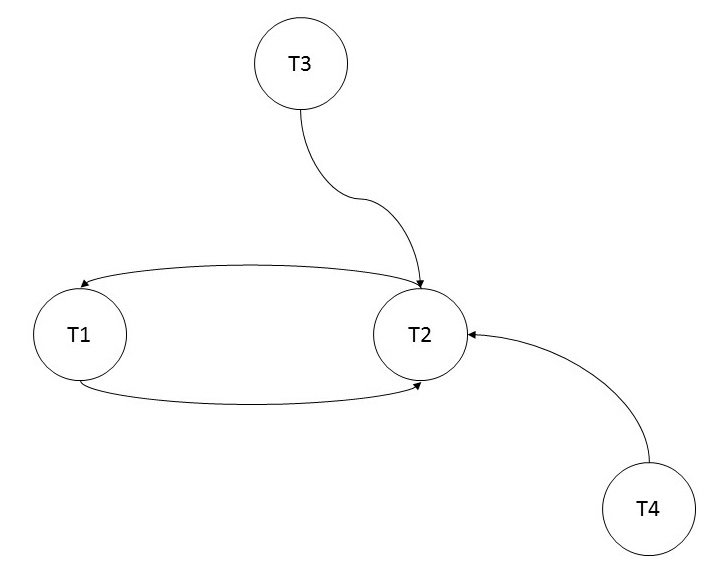
\includegraphics[scale=0.2]{img/wait_graph}
		\caption{Wait graph with a deadlock.}
	\end{figure}
}\end{slide}

\SlideSection{Tasks}
\SlideSubSection{Task 1}
\begin{slide}{
	\item List all the possible conflicts arising in the transaction schedule below.
	\item Convert the schedule into an equivalent strict 2PL schedule.
	\begin{table}
		\tiny
		\begin{tabular}{l|l}
			T1 & T2\\
			\hline
			R(A) & \\
			R(C) & \\
			W(C) & \\
			& R(B) \\
			& W(B) \\
			& R(C) \\
			& W(C) \\
			Commit & \\
			& Commit \\		
		\end{tabular}
	\end{table}	
	
}\end{slide}

\SlideSubSection{Solution}
\begin{slide}{
	\item The only conflict is a dirty read on C in T2.
	\begin{table}
		\tiny
		\begin{tabular}{l|l}
			T1 & T2\\
			\hline
			S(A) & \\
			R(A) & \\
			X(C) & \\
			R(C) & \\
			W(C) & \\
			& X(B) \\
			& R(B) \\
			& W(B) \\
			& WaitLock(C) \\
			Commit & \\
			Unlock(A) & \\
			Unlock(C) & \\
			& X(C) \\
			& R(C) \\
		 	& W(C) \\
			& Commit \\
			& Unlock(B) \\
			& Unlock(C) \\	
		\end{tabular}
	\end{table}	
}\end{slide}

\SlideSubSection{Task 2}
\begin{slide}{
	\item List all the possible conflicts arising in the transaction schedule below.
	\item Convert the schedule into an equivalent strict 2PL schedule.
	\begin{table}
		\tiny
		\begin{tabular}{l|l|l}
			T1 & T2 & T3\\
			\hline
			W(A) & & \\
			& R(A) & \\
			& W(A) & \\
			& W(B) & \\
			& Commit & \\
			& & W(A) \\
			& & R(B) \\
			& & W(C) \\
			W(B) & & \\
			Commit & & \\
			& & R(C) \\
			& & W(A) \\
			& & Commit\\	
		\end{tabular}
	\end{table}	
	
}\end{slide}

\SlideSubSection{Solution}
\begin{slide}{
	\item There is a dirty read conflict on A between T1 and T2.
	\item There is a lost updated conflict on A between T1 and T3.
	\item There is an unrepeatable read conflict on B between T3 and T1.
	\item Note that there is NO dirty read conflict on B between T2 and T3 because T2 commits before T3 reads B.
}\end{slide}

\SlideSubSection{Solution}
\begin{frame}[fragile]{Tasks}
	\begin{table}
		\tiny
		\begin{tabular}{l|l|l}
			T1 & T2 & T3\\
			\hline
			X(A) & & \\
			W(A) & & \\
			& WaitLock(A) &\\
			& & WaitLock(A) \\
			X(B) & & \\
			W(B) & & \\
			Commit & & \\
			Unlock(A) & & \\
			Unlock(B) & & \\
			& X(A) & \\
			& R(A) & \\
			& W(A) & \\
			& X(B) & \\
			& W(B) & \\
			& Commit & \\
			& Unlock(A) & \\
			& Unlock(B) & \\
			& & X(A) \\
			& & W(A) \\
			& & S(B) \\
			& & R(B) \\
			& & X(C) \\
			& & W(C) \\
			& & R(C) \\
			& & W(A) \\
			& & Commit\\
			& & Unlock(A) \\
			& & Unlock(B) \\
			& & Unlock(C) \\	
		\end{tabular}
	\end{table}	
\end{frame}	
	

\end{document}

\begin{slide}{
\item ...
}\end{slide}

\begin{frame}[fragile]
\begin{lstlisting}
...
\end{lstlisting}
\end{frame}
